% $Id: ESMF_archoverview.tex,v 1.5 2003/05/07 22:04:07 jwolfe Exp $

\section{Architectural Overview}
\label{sec:ArchOver}
The ESMF architecture is characterized by the layering strategy shown in figure \ref{fig:TheESMFwich}. In this architectural pattern user code components that implement the {\it science} elements of an algorithm, for example evaluating
finite-difference calculations or radiation physics terms, are sandwiched between two layers. The upper layer is
denoted the {\bf Superstructure} layer and the lower layer the {\bf Infrastructure} layer. The role of the {\bf Superstructure}
layer is to provide a shell which encompasses user code and provides a context for interconnecting input and output
data streams between components. The key elements of the {\bf Superstructure} layer are described in section \ref{sec:superstructure}.
These elements include the extensible classes that represent envelope user code components, ensuring that all
components present consistent interfaces. The {\bf Infrastructure} layer provides a foundation that developers of
user components can use to speed construction and to ensure consistent, guaranteed behavior of components.
The elements of the {\bf Infrastructure} layer include constructs to support parallel processing with data types tailored
to Earth science applications, specialized libraries to support consistent time and calendar management and
performance, error handling and scalable I/O tools. The {\bf Infrastructure} layer is described in section \ref{sec:infrastructure}.
A hierarchical combination of {\bf Superstructure}, user code components and Infrastructure are joined together
to form what is termed an {\it application component} in the ESMF programming paradigm.

\subsection{Programming Paradigm}
A complete, executable assembly of {\bf Superstructure}, user code components and {\bf Infrastructure} collectively forms an ESMF {\it application component}.
Figure \ref{fig:ESMFApplication} shows the generic structure of an ESMF application component. 
This figure shows a single tier composition involving three components. It captures the essence of the composition based programming paradigm that 
ESMF employs, multi-tier composition is also supported in which components are recursively nested.
An application is composed by connecting together one or more
numerical simulation or other user code components within an overall ESMF based environment, figure \ref{fig:ESMFApplication} (1). User code components, figure \ref{fig:ESMFApplication} (3), are written
or modified to fit within the ESMF environment that envelopes
the user code components and that supports a unified high-level {\bf Superstructure} for connecting data and control flows between 
components. A foundation-level {\bf Infrastructure} is also provided, figure \ref{fig:ESMFApplication} (2),
to both accelerate user code development and ensure compatibility
and consistency between components and between hardware platforms. 
\begin{center}
\begin{figure}
\caption{The ESMF programming paradigm defines how an overall application is constructed. An application is an assembly
of one or more gridded and coupler components (1). Components may make use of the ESMF {\bf Infrastructure} toolkit (2). All components,
gridded components, coupler components and the top-level application component are primarily user written (3).}
\label{fig:ESMFApplication}
\scalebox{.5}{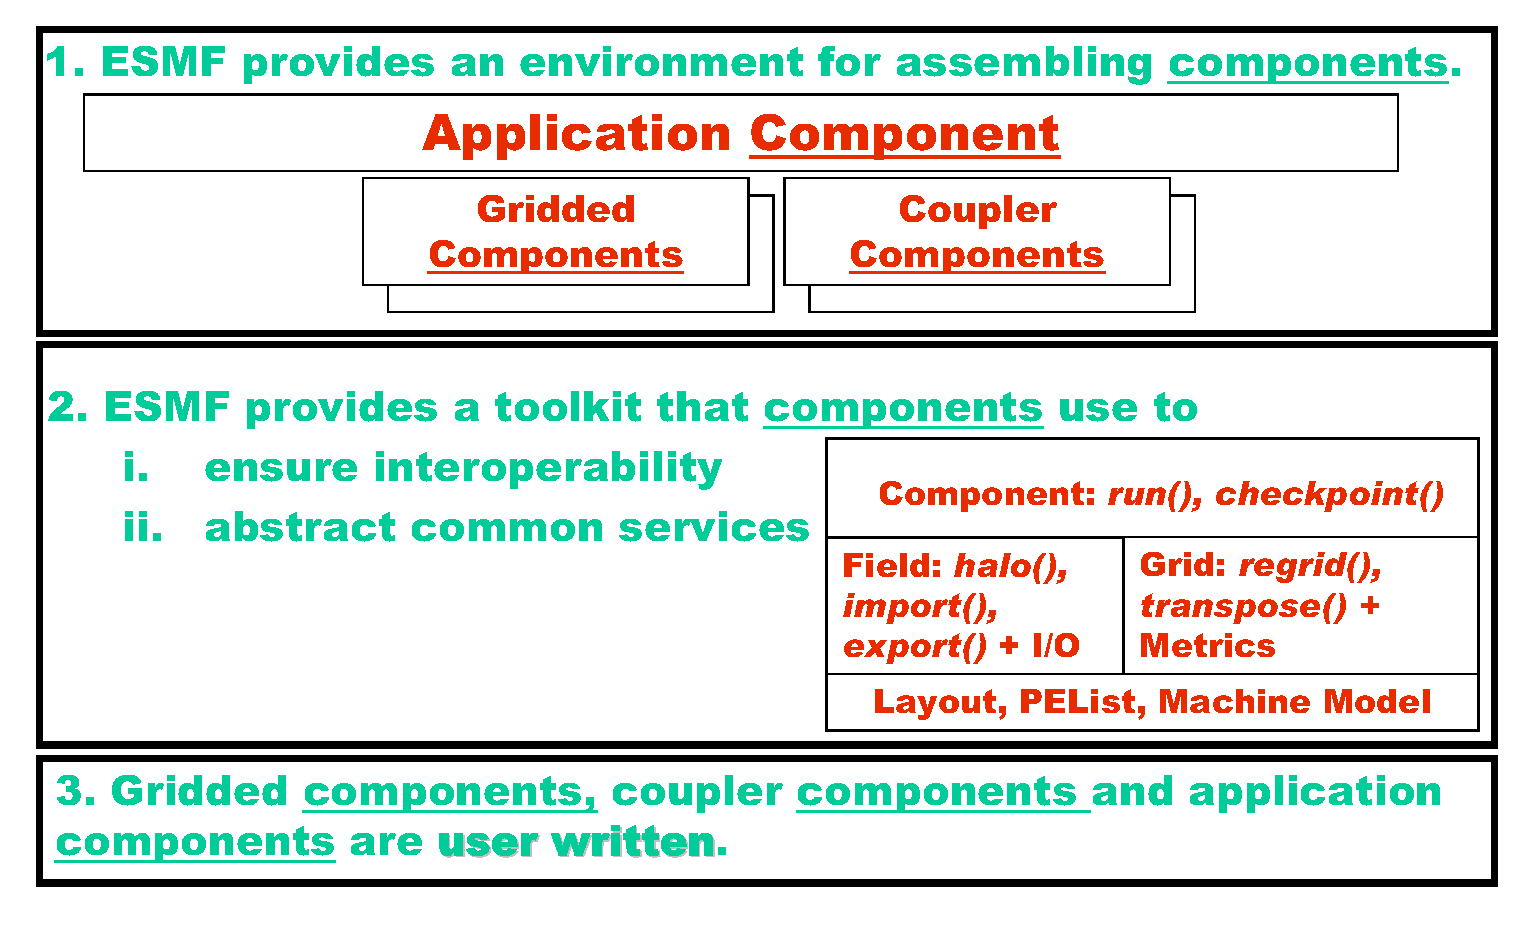
\includegraphics{ESMFprogrammingparadigm.eps}}
\end{figure}
\end{center}

\subsection{Superstructure}
\label{sec:superstructure}
The ESMF {\bf Superstructure} layers in an application furnish a unifying context within which user components are interconnected. For 
example an atmospheric model may use a particular land-surface model in calculating simulated evaporative fluxes. 
The flow of data and sequence of computation between atmospheric model term evaluations and land-surface model
term evaluations would be prescribed in the {\bf Superstructure} layer. Under ESMF user code components are constructed or adapted
to fit within this {\bf Superstructure} layer. This ensures that large components can be interchanged. There may still be issues
of physical consistency between components, but ensuring that all components comply with the requirement to fit
within an ESMF {\bf Superstructure} layer eliminates computational incompatibilities. 

The {\bf Superstructure} layer provides
the foundation for a flexible mechanism to address physical consistency between components that may use different dimensions or units to represent the
same quantity or that may partition physical data differently. Classes called {\it Gridded Components}, 
{\it Coupler Components}, {\it Import States} and {\it Export States} are used within the {\bf Superstructure} layer
to achieve this flexibility.
We describe these classes below:

\subsubsection{Import and Export State Classes}
User code components under ESMF use special interface objects for component to component data exchanges. These objects are 
of type Import State and Export State. These special types support a variety of methods that allow user code components 
to, for example, fill an export state object with data to be shared with other components or query an import state object to 
determine its contents. In keeping with the overall requirements for high-performance it is permitted for Import State and
Export State contents to use references or pointers to component data, so that costly data copies of potentially
very large data structures can be avoided where possible. The content of an Import State and an Export State is 
self-describing.

\subsubsection{Interface Standards}
The Import State and Export State abstractions are designed to be flexible enough
that ESMF does not need to mandate a single standard for fields. For example ESMF does not prescribe the units
of quantities exported or imported, instead it provides mechanics to describe the units, memory layout, grid coordinates 
of the fields in Import States and Export States.  This allows the ESMF software to support a range of different policies for
physical fields. The interoperability experiments that we are using to demonstrate ESMF make use of the emerging
CF standards \cite{ref:CF} for describing physical fields. This is a policy choice for that set of experiments. The ESMF 
software itself can support arbitrary conventions for labeling and characterizing the content of Import and 
Export States.

\subsubsection{Gridded Component Class}
The Gridded Component class is used to for a user component that takes in one Import State and produces one
Export State, both based on the same discrete grid. Examples of Gridded Components are major Earth system 
model components such as land-surface models, ocean models, atmospheric models and sea-ice models. Components 
used for linear algebra manipulations in a state-estimation or data-assimilation optimization procedure are also 
created as Gridded Components. In general the Import State and the Export State of a Gridded Component will 
use the same base discrete grid.

\subsubsection{Coupler Component Class}
The other top-level component class supported in the current ESMF architecture is a Coupler Component class.
This class is used for components that take one or more Import States as input and map them through
spatial and temporal interpolation or extrapolation onto an output Export State. In a Coupler Component
it is often the case that the output Export State is on a different base discrete grid to that of
the Import State(s). The role of Coupler Components is generally mapping the Export States from one or
more Gridded Components to the Import State of another Gridded Component. For example, in a coupled
ocean-atmosphere simulation a Couple Component would be used to map a set of sea-surface fields 
in an ocean model to appropriate planetary boundary layer fields in an atmospheric model.
\subsubsection{Flexible data and control flow}
Import States, Export States, Gridded Components and Coupler Components can be arrayed flexibly
within a {\bf Superstructure} layer. Using these constructs it is possible to configure a set of concurrently
executing Gridded Components joined through a single Coupler Component of the style shown in figure 
\ref{fig:hubspoke}. Is is also possible to configure a set of sequentially executing components with multiple
pair-wise Coupler Components defined to support individual Gridded Component to Gridded 
Component mappings independently, figure \ref{fig:point2point}.

\begin{figure}
\caption{ESMF can support configurations with a single central Coupler Component. In this case inputs from all Gridded 
Components are transferred and regrided between all components in one place. The block arrows show how the 
Coupler Component 
(symbolized by the star icon) must take inputs from all Gridded Components (symbolized by the model output images) 
and return data to all Gridded Components.}
\label{fig:hubspoke}
\scalebox{0.7}{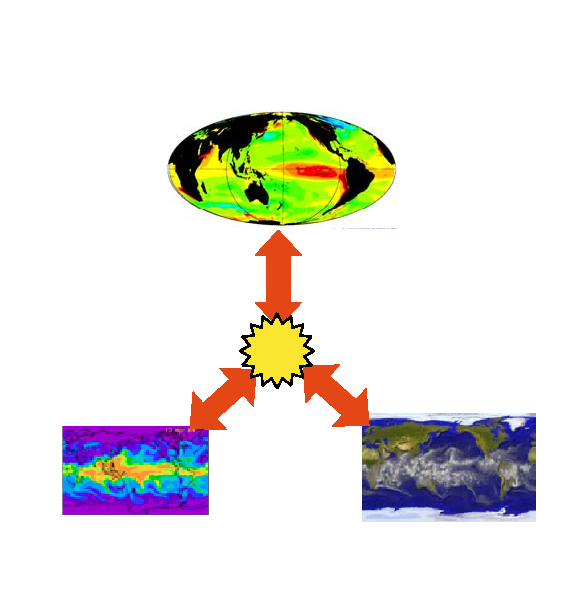
\includegraphics{couplings_hub_and_spoke.eps}}
\end{figure}

\begin{figure}
\caption{ESMF also supports configurations with multiple point to point Coupler Components. 
These take inputs from one Gridded
Component and transfer and regrid the data for passing to another Gridded Component. The block arrows show the
flow of data between point to point pairings of Coupler Components (symbolized by the star icons) and Gridded 
Components (symbolized by the model output images).}
\label{fig:point2point}
\scalebox{0.7}{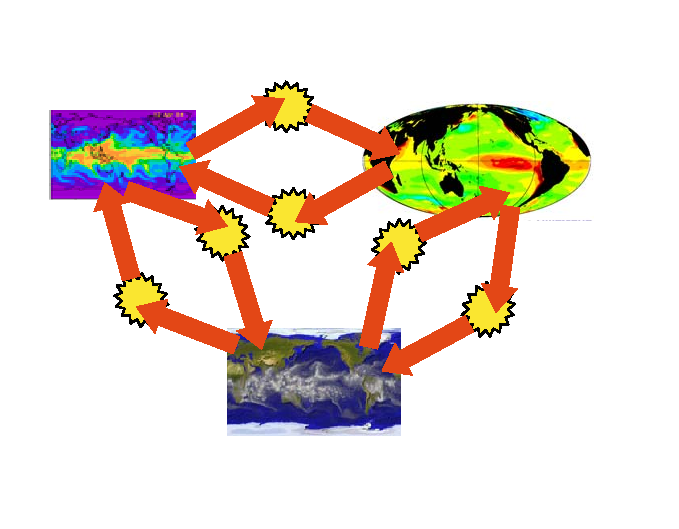
\includegraphics{couplings_pt_to_pt.eps}}
\end{figure}

The set of {\bf Superstructure} abstractions allows flexible data-flow and control between components. However, 
components will often use different discrete grids, and time-stepping components may march forward with different time
intervals. In a parallel compute environment different components may be distributed in a different manner on the
underlying compute resources. The ESMF {\bf Infrastructure} layer provides elements to manage this complexity.

\subsection{Infrastructure}
\label{sec:infrastructure}
Figure \ref{fig:threecomponents} illustrates three Gridded Components that use three different grids being coupled together. In 
order to achieve this coupling several steps beyond defining {\bf Superstructure} Import State and Export State objects to act
as data conduits are required. Coupler Components are required that can map between the different
grids, this mapping may also involve mapping between different units and/or memory layout conventions for the fields that
pass between components. In a parallel compute environment the Coupler Components may also be required to map between different 
domain decompositions. In order to advance in time correctly the separate Gridded Components must have compatible notions
of time. Approaches to parallelism within the Gridded Components must also be compatible. The {\bf Infrastructure} layer
contains a set of classes that address these issues and assist in managing overall system complexity. We describe
these classes below:

\begin{figure}
\caption{Schematic showing the coupling of components that use different discrete grids and different time-stepping. 
In this example component {\it NCAR Atmosphere} might use a spectral grid based on spherical harmonics, component
{\it GFDL Ocean} might use a latitude-longitude grid but with a patched decomposition that does not include
land masses and component {\it NSIPP Land} might use a mosaic based grid for representing vegetation patchiness
and a catchment area based grid for river routings. The {\bf Infrastructure} layer contains tools to help develop 
software for coupling between components on different grids, mapping between components with different distributions in a 
multi-processor compute environment and to synchronize events between components with different time-stepping intervals 
and algorithms.  }
\label{fig:threecomponents}
\scalebox{0.5}{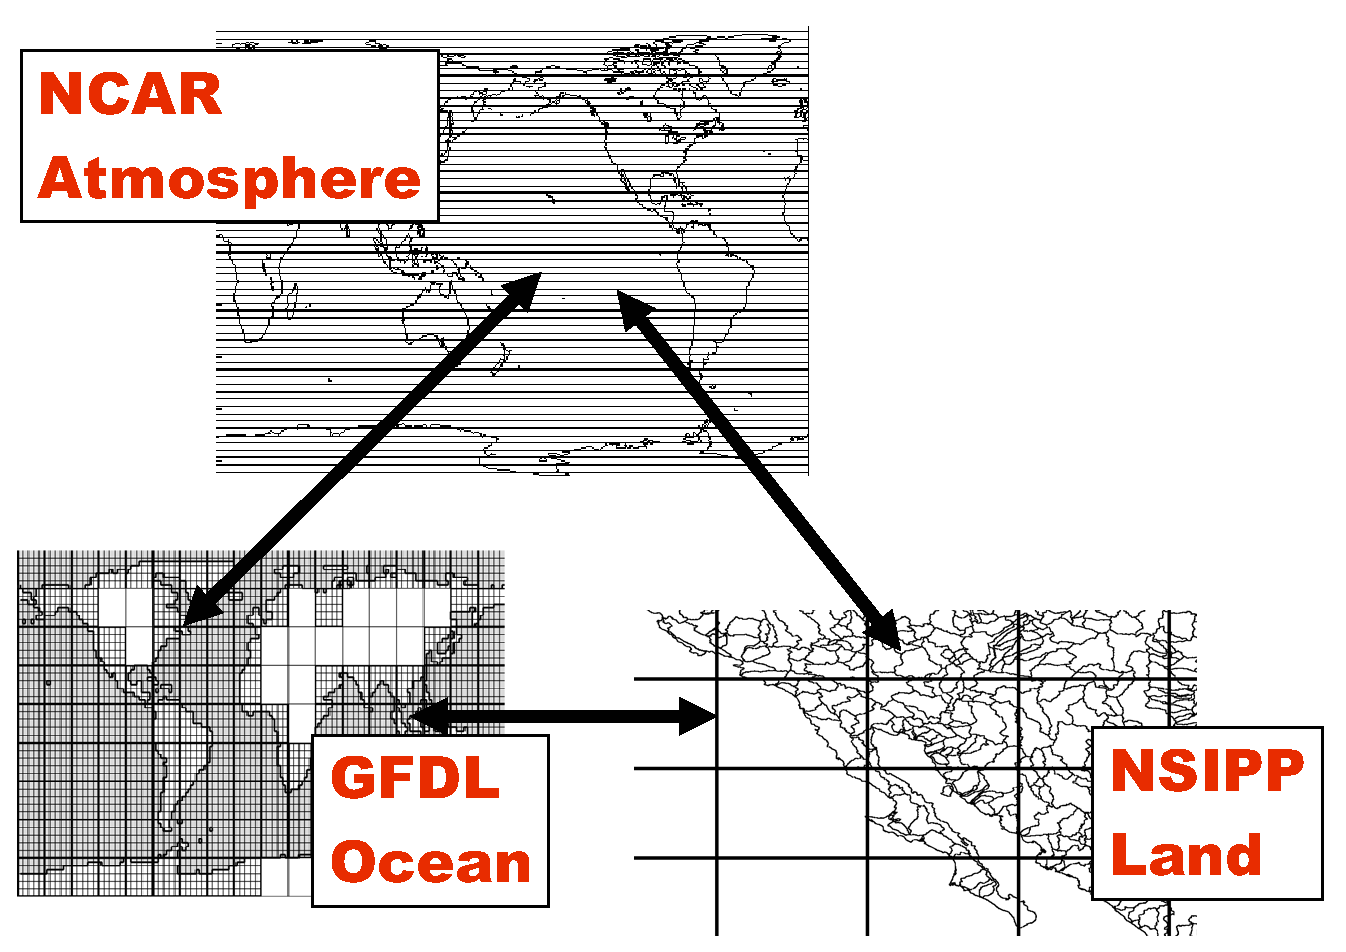
\includegraphics{regrid.eps}}
\end{figure}

\subsubsection{Field and Array Classes}
The {\it Field} and {\it Array} classes contain data together with descriptive
physical and computational attribute information. The physical attributes include information that describes the units
of the data. The computational attributes include information on the layout in memory of the field data. The Field class
is primarily geared toward structured data. A comparable class called {\it Location Stream} provides a self-describing
container for unstructured observational data streams.

\subsubsection{Physical Grid Class}
The {\it Physical Grid} class is an extensible class that holds discrete grid information. It has subtypes that allow
it to serve as a container for the full range of different physical grids that might arise in a coupled system.
In the example in figure \ref{fig:threecomponents} objects of type Physical Grid would hold grid information for
each of the spectral grid, the latitude-longitude grid, the mosaic grid and the catchment grid. 

\subsubsection{Regrid Class}
The {\it Regrid} class is an extensible class that allows conservative remapping between a field on one physical grid
to a field on a different physical grid \cite{ref:SCRIP}. It supports precomputation of grid interpolation weights and allows user selectable
corrections for global or local conservation requirements. Regrid is designed to be scalable on parallel platforms.
When mapping between grids
the Regrid class utilizes the Physical Grid object and Field and Array objects.

\subsubsection{Distributed Grid Class}
The {\it Distributed Grid} class is used to represent the decomposition of a data structure into sub-domains, typically for
parallel processing purposes. The class is designed to support a generalized ``ghosting'' for tiled 
decompositions of finite difference, finite volume and finite element codes. 

\subsubsection{Time and Calendar Management Class}
To support synchronization between components {\it Time} and {\it Calendar} classes along with an associated
{\it Clock} class are provided. These classes allow Gridded and Coupler Component processing
to be latched to a common controlling clock.

\subsubsection{I/O Classes}
The {\bf Infrastructure} layer defines a set of {\it I/O} classes for storing and retrieving Field and Grid information
to and from persistent storage. The I/O classes support a range of standard formats including binary I/O and netCDF, HDF5 and
GRIB based I/O.

\subsubsection{Communication Class}
To provide a mechanism for ensuring performance portability ESMF defines a {\it Communication} class. This class provides a set of
high-level platform independent interfaces to performance critical parallel processing communication routines. These routines can be tuned
to specific platforms to ensure optimal parallel performance on many platforms. The Communication class includes reduction
operations, transpose or redistribution operations and halo or ghost operations.

\subsubsection{Logging and Profiling Class}
The {\it Logging} and {\it Profiling} classes are designed to aid in managing the complexity of multi-component applications. They provide
ESMF with a unified mechanism for notification messages, for timing and counting events.





